\documentclass{standalone}
\standaloneconfig{border=2mm 2mm 2mm 2mm}
%Packages & Libraries
\usepackage{tikz}
\usepackage{gensymb}
\usepackage{textcomp}
\usetikzlibrary{calc}

\begin{document}

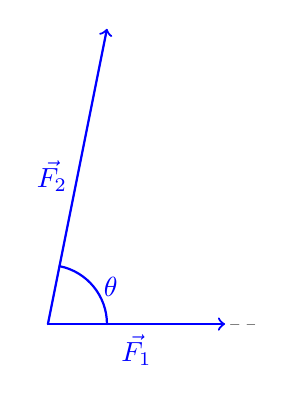
\begin{tikzpicture}[line cap=round,scale=0.75]
    % Axes
    \draw[dashed,gray] (0,0) -- (3.5,0); %x    
    % Define the origin
    \coordinate (O) at (0,0);    
    % Define vectors F1 and F2
    \coordinate (A) at (3,0); % Vector F1
    \coordinate (B) at (1,5); % Vector F2
    % Draw vector F1
    \draw[->, thick, blue] (O) -- (A) node[midway, below] {$\vec{F_1}$};
    % Draw vector F2 
    \draw[->, thick, blue] (O) -- (B) node[midway, left] {$\vec{F_2}$};
    \draw[thick, blue] (1,0) arc (0:78.69:1) node[midway, right]{$\theta$};   
\end{tikzpicture}

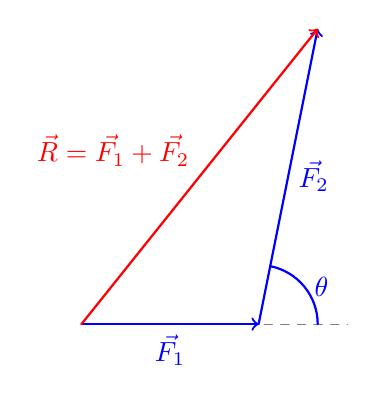
\begin{tikzpicture}[line cap=round,scale=0.75]
    % Axes
    \draw[dashed,gray] (0,0) -- (4.5,0); %x
    % Define the origin
    \coordinate (O) at (0,0);    
    % Define vectors F1 and F2
    \coordinate (A) at (3,0); % Vector F1
    \coordinate (B) at (1,5); % Vector F2
    % Draw vector F1
    \draw[->, thick, blue] (O) -- (A) node[midway, below] {$\vec{F_1}$};
    % Draw vector F2 starting from the tip of F1
    \draw[->, thick, blue] (A) -- ($(A)+(B)$) node[midway, right] {$\vec{F_2}$};
    \draw[thick, blue] (4,0) arc (0:78.69:1) node[midway, right]{$\theta$};
    % Draw the resultant vector R = F1 + F2 from origin
    \draw[->, thick, red] (O) -- ($(A) + (B)$) node[midway, above left] {$\vec{R} = \vec{F_1} + \vec{F_2}$}; 
\end{tikzpicture}

\end{document}
